\documentclass[12pt]{article}
\usepackage[a4paper, margin=1in]{geometry}
\usepackage{graphicx}
\usepackage{hyperref}

\title{Title}
\author{Marco Coppola,\\
Valerio Pio De Nicola,\\
Davide De Rosa \\ \\
University of Bologna}
\date{}

\begin{document}

\maketitle

\begin{abstract}
per la fine
\end{abstract}

\section{Introduction}
per la fine

\section{InstructLab}
\subsection{Introduction to LAB}
Large language models (LLMs) have achieved success in NLP tasks due to the transformer architecture, which enables training on vast amounts of unstructured data. LLM training consists of two main phases: \textbf{pre-training} (which is computationally expensive and involves predicting the next token using massive datasets) and \textbf{alignment tuning} (which refines model behavior through instruction and preference tuning).\vspace{14pt}\\
Pre-training dominates the resource cost, while alignment tuning, including instruction tuning (training on task-specific instructions) and preference tuning (using human feedback methods like RLHF), requires significantly fewer data and compute resources.\\
Despite this, alignment tuning is crucial for optimizing LLMs for real-world use.\vspace{14pt}\\
To address challenges in scaling alignment tuning, the \textbf{LAB} (\textbf{Large-scale Alignment for chatBots}) \textbf{method} is introduced. LAB includes:
\begin{enumerate}
    \item \textbf{Synthetic data generation} guided by taxonomy and quality assurance, avoiding reliance on proprietary LLMs or extensive human curation.  
    \item \textbf{A novel multi-phase training framework} that integrates new knowledge without causing catastrophic forgetting.
\end{enumerate}
LAB-trained models achieve competitive performance compared to those using human-annotated or GPT-4-generated data, demonstrating its effectiveness for improving LLM instruction-following capabilities.\vspace{14pt}\\
Recent advancements in instruction tuning for large language models (LLMs) have primarily relied on two key methodologies: \textbf{human-annotated datasets} and \textbf{synthetic data generation}. Traditional approaches, such as those pioneered by OpenAI and later adopted by the creators of LLaMA 2, emphasize the collection of high-quality human-generated data. This process involves extensive human annotation efforts, requiring rigorous selection and training of annotators to ensure consistency and quality.\vspace{14pt}\\
While effective in aligning models with human preferences, these methods are resource-intensive, costly, and often slow, limiting the ability to rapidly explore new instruction types and model capabilities.
To address these limitations, synthetic data generation has emerged as an alternative, leveraging LLMs to produce instruction-tuning datasets.\vspace{14pt}\\
Early efforts, such as Self-Instruct, introduced a bootstrapping approach that expands a small set of human-written seed instructions into a large dataset using an LLM’s own generation capabilities. Subsequent refinements sought to enhance data diversity and instruction complexity through iterative and principled augmentation techniques.\\
Other works have further extended this approach by focusing on task diversity and progressive training frameworks, incorporating richer reasoning signals to improve model performance incrementally.\vspace{14pt}\\
More recently, semi-automated techniques, such as GLAN, have introduced a structured approach to synthetic data generation by leveraging human-curated taxonomies.\\
However, such methods remain constrained by the limitations of the teacher model used for data generation, particularly when relying on proprietary models like GPT-4, which impose restrictions on the commercial usability of the generated data.\vspace{14pt}\\
In contrast, open-source approaches, such as LAB, attempt to mitigate these concerns by employing models like Mixtral, allowing for greater flexibility in data generation and application.\vspace{14pt}\\
The ongoing evolution of instruction tuning methods highlights the trade-offs between human-annotated and synthetic data-driven approaches.\\
While human-generated data ensures high-quality alignment, it is costly and inflexible.\\
Conversely, synthetic data techniques offer scalability and efficiency but introduce challenges related to data diversity, quality control, and legal constraints surrounding proprietary models.\\
Future research will likely focus on hybrid approaches that balance these trade-offs, incorporating the strengths of both methodologies to enhance the instruction-tuning process.

\subsection{How does LAB work}
LAB is a structured framework designed to enhance instruction tuning through a combination of systematic data curation and multi-phased training. It consists of two key components:
\begin{itemize}
    \item \textbf{Taxonomy-Guided Synthetic Data Generator}: this component facilitates data curation by organizing instructions into a structured taxonomy. It also plays a crucial role in guiding the synthetic data generation process, ensuring both high diversity and quality in the instruction-tuning dataset. By leveraging a well-defined taxonomy, LAB aims to improve the comprehensiveness and relevance of the generated data.
    \item \textbf{Multi-Phased Instruction-Tuning with Replay Buffers}: to maintain training stability and mitigate issues such as catastrophic forgetting, LAB employs a multi-stage tuning approach. The use of replay buffers allows the model to retain previously learned information while adapting to new instructions, thereby improving overall alignment performance.
\end{itemize}
Together, these components form an end-to-end pipeline for aligning a pre-trained LLM, as illustrated in Figure~\ref{fig:ilab}. This approach balances synthetic data diversity with training stability, making it a scalable and effective method for large-scale instruction tuning.\\
\begin{figure}
    \centering
    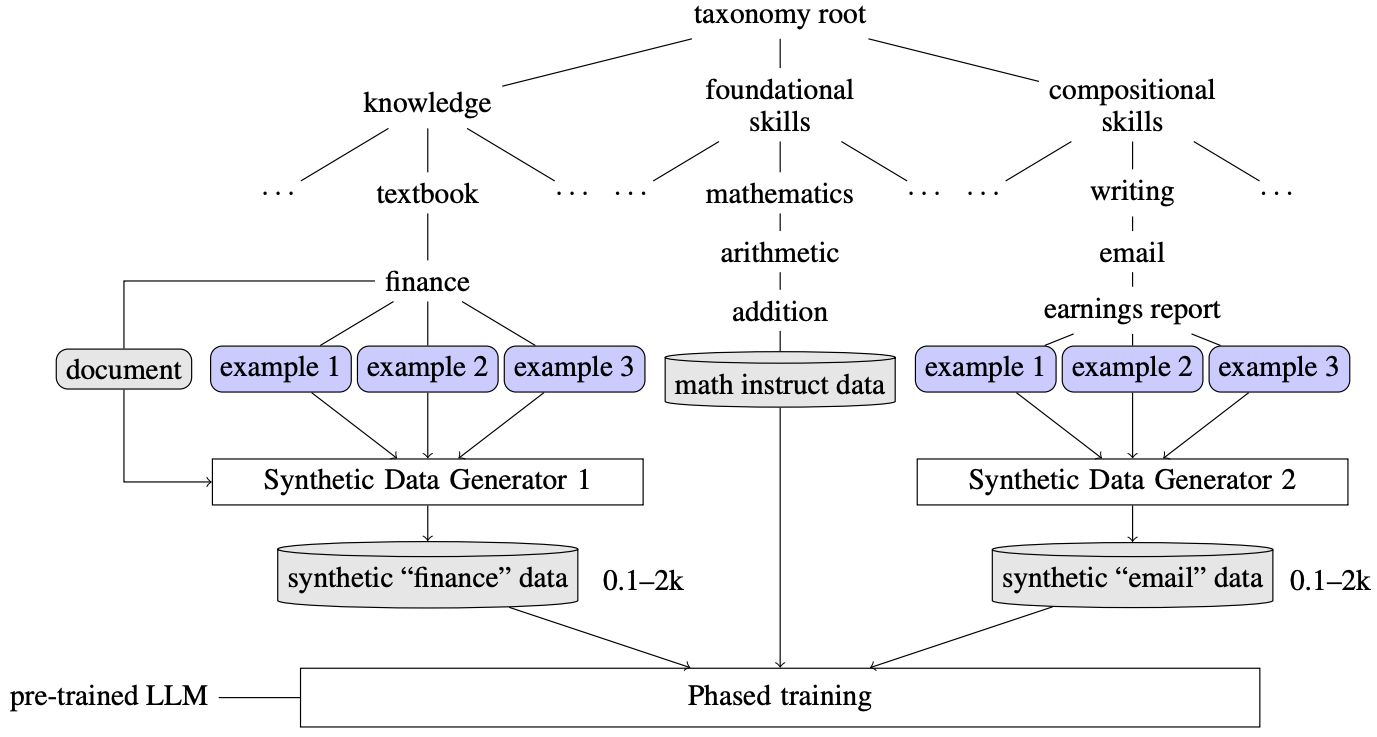
\includegraphics[width=1\textwidth]{img/figure1.png}
    \caption{\textit{Overview of the LAB alignment method. Starting from the taxonomy root, data are curated in each top-level groups and examples in the leaf nodes are used by the synthetic data generators to generate orders of magnitude data for the phased-training step for instruct-tuning.}}
    \label{fig:ilab}
\end{figure}

\subsubsection{Taxonmy}
LAB's taxonomy serves as a structured framework for organizing instruction-tuning data, enabling systematic curation and enhancement of training datasets. It hierarchically classifies data samples into three main branches: \textbf{knowledge}, \textbf{foundational skills}, and \textbf{compositional skills}. Each of these branches is further subdivided into more granular levels, with specific tasks defined at the leaf nodes. These leaf nodes are exemplified by manually written instruction-response pairs, ensuring clarity in task representation.\vspace{14pt}\\
This hierarchical organization provides several advantages.\vspace{14pt}\\
First, it allows model designers and data curators to identify gaps in the model’s capabilities by pinpointing missing or underrepresented tasks.\vspace{14pt}\\
Second, it facilitates the incremental expansion of training data, as new tasks can be seamlessly integrated by adding a leaf node under the appropriate branch, accompanied by 1–3 examples.\vspace{14pt}\\
This structured approach ensures that instruction tuning remains both comprehensive and adaptable, improving the overall alignment and robustness of the trained LLM.\vspace{14pt}\\
\textbf{Knowledge}\\
The \textit{Knowledge} branch in LAB’s taxonomy is structured to systematically classify and curate domain-specific information. It is first categorized based on document types, such as textbooks, technical manuals, and research papers. These categories are further subdivided into specific domains, including finance, statistics, and other specialized fields (illustrated in Figure~\ref{fig:ilab}). Each domain contains a curated set of documents alongside a sample collection of domain-specific questions and answers, ensuring a well-organized knowledge repository.\vspace{14pt}\\
A key advantage of this hierarchical structure is the ability to exercise control over the licensing of text documents used in synthetic data generation. Only documents with permissible licenses are selected, while unlicensed or restricted content is excluded. This approach enhances the integrity and compliance of the synthetic data pipeline, ensuring that knowledge-based instruction tuning is conducted ethically and legally.\vspace{14pt}\\
\textbf{Foundational Skills}\\
The \textit{Foundational Skills} branch in LAB’s taxonomy encompasses core capabilities that serve as the building blocks for advanced knowledge acquisition and compositional reasoning. These skills include mathematics, coding, linguistic ability, and reasoning, all of which are essential for enhancing the model’s overall learning capacity. Mastering these foundational skills enables the model to generalize more effectively across diverse tasks and domains.\vspace{14pt}\\
To instill these competencies, LAB leverages publicly available datasets, ensuring that the training data remains transparent and accessible. The hierarchical organization of this branch, illustrated in Figure~\ref{fig:ilab}, allows for structured expansion of foundational skills by incorporating new datasets and refining instruction-response pairs\\
This method ensures that the model is well-equipped to build upon fundamental knowledge, facilitating more complex reasoning and problem-solving in subsequent training phases.\vspace{14pt}\\
\textbf{Compositional Skills}\\
The \textit{Compositional Skills} branch in LAB’s taxonomy encompasses tasks that require the integration of knowledge and foundational skills to handle complex, multi-step queries effectively. Unlike isolated knowledge recall or basic skill application, compositional skills demand a synergistic approach, where the model combines various competencies to generate coherent and contextually appropriate responses.\vspace{14pt}\\
For example, crafting a company-wide email that summarizes last quarter’s performance and provides guidance for the upcoming year requires multiple capabilities: financial knowledge (understanding revenue, profit, and loss), mathematical reasoning (basic arithmetic for calculations), and linguistic proficiency (formal business communication). This category ensures that the model can synthesize information from different domains, demonstrating adaptability and depth in response generation.\vspace{14pt}\\
By structuring compositional skills within the taxonomy, LAB enables targeted training on multi-faceted tasks, ensuring the model can navigate complex real-world queries with precision and coherence.

\subsubsection{Taxonomy-Driven Synthetic Data Generator}
LAB enhances \textbf{synthetic data generation} (\textbf{SDG}) by leveraging a \textit{taxonomy-driven approach} rather than relying on traditional random sampling methods.\\
While manually curated data samples embedded in the taxonomy’s leaf nodes can be used for direct instruction tuning, prior research suggests that a large volume of high-quality instruction data is necessary for improving instruction-following capabilities in LLMs.\vspace{14pt}\\
Existing SDG methods attempt to scale synthetic data generation using teacher models, but they suffer from mode collapse—over-representing the dominant patterns of the teacher model while neglecting diverse or less common instruction types.\vspace{14pt}\\
This limitation arises from random selection of seed examples, which results in prompts that reflect an "average" of the dataset rather than task-specific examples. Consequently, the teacher model generates synthetic data that predominantly aligns with its dominant distribution while ignoring the long-tail of diverse or nuanced tasks. To overcome this, LAB replaces random selection with taxonomy-driven sampling, ensuring that data generation is targeted at the level of individual leaf nodes. This approach guarantees balanced representation across different instruction types, preventing bias toward a subset of commonly occurring prompts.\vspace{14pt}\\
LAB introduces two new SDG methods based on this taxonomy-guided framework:
\begin{enumerate}
    \item \textbf{Skills Generation}: this method uses the task examples stored in the leaf nodes to generate a larger dataset using the open-source \textbf{Mixtral-7x8B model}. By focusing on specific skill categories, LAB ensures better diversity and task-specific representation** in the synthetic data.  
    \item \textbf{Knowledge Generation}: unlike prior approaches that rely on a teacher model’s internal knowledge, LAB’s knowledge generation method still employs \textbf{Mixtral-7x8B}, but without depending on pre-existing knowledge stored in the model. This approach mitigates biases introduced by the teacher model’s knowledge limitations while maintaining control over the source material used for synthetic data creation.  
\end{enumerate}
By structuring data generation around the taxonomy, \textbf{LAB improves both the diversity and quality} of synthetic instruction-tuning datasets, addressing key weaknesses in traditional SDG pipelines.\vspace{14pt}\\
\textbf{Skill Generation}\\
Skills-SDG employs a structured, multi-stage approach to generate high-quality instruction data while maintaining diversity and alignment with human expectations. This process is driven by four specialized prompt templates, each defining a distinct role for the teacher model (Mixtral-7x8B) as either a generator or an evaluator. These carefully designed prompts enforce specific principles and constraints at each stage, ensuring that the generated dataset remains relevant, diverse, and high quality:
\begin{enumerate}
    \item \textbf{Instruction Generation}: in the first stage, the teacher model functions as a question generator, using a specialized prompt to systematically traverse the taxonomy’s leaf nodes and generate a broad set of diverse, targeted instructions. This ensures comprehensive exploration of the domain, avoiding redundancy while maximizing instructional diversity. The principles embedded in the prompt guide the model to produce clear, well-structured, and meaningful queries aligned with human expectations.
    \item \textbf{Evaluating Synthetic Instructions}: once generated, the synthetic instructions undergo a rigorous evaluation process where the teacher model transitions into the role of an instruction evaluator.\\
    Using a set of targeted prompts, the model filters out instructions that are irrelevant to the domain, contain harmful or biased content, or exceed the capabilities of a language model (e.g., requiring real-world actions).\\
    By enforcing strict filtering criteria, this stage ensures that only high-quality and contextually appropriate instructions proceed to the next phase.
    \item \textbf{Generating Responses}: at this stage, the teacher model acts as a response generator, adopting a dual-persona strategy to ensure response quality matches task-specific expectations. Using distinct prompts, the model generates creative and open-ended responses for domains such as writing and role-play, and precise, structured answers for STEM subjects and data extraction tasks.\\
    This tailored approach aligns responses with human-like reasoning and domain-specific constraints, enhancing naturalness and usability.
    \item \textbf{Evaluating Instruction-Response Pairs}: in the final stage, the teacher model conducts quality assurance by rigorously evaluating each instruction-response pair. Using a 3-point rating system, the model filters out incorrect or factually inaccurate responses, off-topic or low-relevance instructions, and samples that violate predefined principles (e.g., harmful or misleading content).\\
    This ensures that only high-quality, well-aligned data is incorporated into the student model's training dataset, leading to more reliable and effective instruction-following capabilities.
\end{enumerate}
By structuring Skills-SDG around taxonomy-driven prompts and multi-stage validation, LAB overcomes the limitations of random sampling in SDG, ensuring that the generated dataset is diverse, high-quality, and well-aligned with instructional objectives. This method enhances both the robustness and adaptability of student models trained on the synthesized data.\vspace{14pt}\\
\textbf{Knowledge Generation}\\
The main limitation of synthetic data generation (SDG) is that it relies heavily on the knowledge and capabilities of the teacher model. This means that if the model lacks information on a particular domain, it cannot effectively generate high-quality synthetic data for that field. That’s why most successful SDG methods today, such as those referenced in recent studies, tend to use powerful models like GPT-4, which have broad knowledge coverage.\vspace{14pt}\\
However, even the most advanced models are not trained on every possible domain, particularly highly specialized or niche areas.\\
To overcome this, researchers at LAB have developed a new approach called \textbf{knowledge-SDG}. Unlike conventional SDG methods that depend solely on the teacher model’s pre-existing knowledge, knowledge-SDG grounds the generation process in external, reliable sources such as documents, manuals, and books. This ensures that the generated data remains accurate and avoids hallucinations, which can be a significant issue in technical or specialized fields.\vspace{14pt}\\
The process works by integrating examples curated within a structured taxonomy and supplementing them with external knowledge sources. Moreover, just as with skills-based SDG, the teacher model is also used as an \textbf{evaluator} to verify that the generated content remains faithful to the source material.\\
This extra validation step ensures the reliability and factual accuracy of the synthetic data, making it more suitable for domains where misinformation or inaccuracies could be particularly problematic.\vspace{14pt}\\
\textbf{Multi-Phase Training}\\
LAB training is structured into two key phases: \textbf{knowledge tuning} followed by \textbf{skills tuning}.\vspace{14pt}\\
In the \textbf{knowledge-tuning phase}, the model is trained on data from the knowledge and foundational skills branches of a structured taxonomy. This process is further divided into two steps based on response length.\\
First, the model is trained on samples with shorter responses, and only after that does it move on to longer responses. This approach aligns with previous research and has been shown to improve overall model performance.\vspace{14pt}\\
Once knowledge tuning is complete, the training moves into the \textbf{skills-tuning phase}. Here, the best-performing model from the previous phase is further trained on the compositional skills branch of the taxonomy. A key challenge in this multi-phase training process is catastrophic forgetting — where the model loses previously learned knowledge when exposed to new information. To mitigate this, a replay buffer is used to retain and incorporate data from the knowledge-tuning phase, ensuring that the model does not lose its foundational learning while acquiring more advanced skills.\\
Empirical results suggest that this structured progression — from foundational knowledge to compositional skills — leads to significantly improved benchmark performance.\vspace{14pt}\\

\end{document}